\documentclass[10pt,a4paper]{article}
\usepackage[T1]{fontenc}
\usepackage[utf8]{inputenc}
\usepackage{lmodern}
\usepackage[margin=22mm]{geometry}
\usepackage{microtype}
\usepackage{graphicx}
\usepackage{booktabs}
\usepackage{tabularx}
\usepackage{array}
\usepackage{xcolor}
\usepackage{listings}
\usepackage{tikz}
\usetikzlibrary{positioning,arrows.meta,fit,backgrounds}
\usepackage[font=small,labelfont=bf]{caption}
\usepackage{subcaption}
\usepackage{enumitem}
\usepackage[hidelinks]{hyperref}

\setlist{itemsep=1pt,topsep=3pt}
\newcommand{\code}[1]{\texttt{#1}}
\definecolor{codebg}{gray}{0.96}
\lstset{basicstyle=\ttfamily\footnotesize,backgroundcolor=\color{codebg},frame=none,
  columns=fullflexible,keepspaces=true,showstringspaces=false,xleftmargin=4pt,xrightmargin=4pt,
  aboveskip=6pt,belowskip=6pt,commentstyle=\color{black!55},keywordstyle=\bfseries}

\title{\textbf{Emulating a Synthesizer Before It Arrives}\\[2pt]
\large Recovering an undocumented CPU from its firmware and running the M-VAVE FM-1\\ in a browser}
\author{Joakim Eriksson\\\small\url{https://github.com/joakimeriksson/fm1-emu}}
\date{Technical report \quad\textperiodcentered\quad 13 October 2026 \quad\textperiodcentered\quad written before validation on hardware}

\begin{document}
\maketitle

\begin{abstract}
\noindent
The M-VAVE FM-1 is a pocket FM synthesizer for which a small community writes its own firmware.
It is built on a JieLi AC791N, a dual-core system-on-chip whose CPU, pi32v2, has no public
instruction-set manual. This report describes, step by step, how an emulator of the whole
instrument was built in five days, before the physical unit had been delivered: recovering the
instruction set from vendor disassembly of 25 firmware images, solving operand encodings as exact
linear models, validating semantics with differential probes in which the vendor compiler's own
constant folding is the oracle, modelling the peripherals the firmwares actually touch, and making
it fast enough for real time with two just-in-time compilers (AArch64 natively, WebAssembly in the
browser). The emulator runs M-VAVE's stock firmware on both cores and fifteen community firmwares
unmodified, takes MIDI in, and is published as a web page. Every performance change was accepted
only if the emulated audio stayed byte-identical across three execution modes. The emulator was
then used as the development platform for a new firmware, \emph{FM-1 SID}, which runs a Commodore~64
tune's 6502 code and a reSID model of the SID chip on the FM-1's CPU. The work was done by one person
directing an AI coding agent; the report closes with how that collaboration was organised and which
rules made its output trustworthy.
\end{abstract}

\section{Introduction}

The M-VAVE FM-1 (Fig.~\ref{fig:page}) is a battery-powered six-operator FM synthesizer with a
240$\times$240 colour screen, 27 keys, 14 buttons, 7 encoders, a MIDI~IN jack and stereo audio.
Its stock sound engine is a port of the msfa/Dexed DX7 core. Because its update channel is USB-MIDI
SysEx with only a CRC check, and because the community had documented its hardware and published a
GPL hardware layer (Felucca), people began writing replacement firmwares within weeks of launch:
drum machines, grooveboxes, ambient generators, a chord harp.

The goal of this project was an emulator accurate enough to run those firmwares
\emph{unmodified}, so that anyone can try a firmware before flashing it, a developer can write one
without the synth on the desk, and the firmwares can be played in a browser. Three facts shaped the
work:

\begin{enumerate}
\item \textbf{The CPU is undocumented.} pi32v2 is JieLi's proprietary 32-bit ISA with
  Blackfin-style algebraic assembly (\code{r0 += r1}, \code{if (r2 != 0) goto L}), variable-length
  encodings of 2, 4 and 6 bytes, dual-issue pairs, predicated blocks and hardware loops. No manual
  exists; the existing Ghidra module is described by its author as ``very early stage''.
\item \textbf{The vendor toolchain is public.} JieLi distributes a Clang/LLVM~4.0.1 fork with a
  pi32v2 back end and an \code{objdump} that disassembles it. It runs only on Linux x86-64; here it
  ran on an Apple-silicon Mac through \code{docker run --platform linux/amd64}.
\item \textbf{There was no hardware.} The FM-1 had been ordered but had not arrived. Everything had
  to be established from published firmware images, the toolchain and the community's notes.
\end{enumerate}

\paragraph{What was built.} A Rust workspace (\code{fm1-isa}, \code{fm1-core}, \code{fm1-soc} and
three front ends) of about 12\,600 hand-written lines of Rust plus a generated decoder table; a native
player (\code{fm1-live}) running the real 240\,MHz clock at 2.6--6.3$\times$ real time; a batch runner
for tests; and a WebAssembly build in an AudioWorklet that runs every firmware at 240\,MHz in a
browser (1.6--3.7$\times$ real time in Node). It boots M-VAVE's own firmware (V13 and V15) with both
cores, and the fifteen community firmwares listed on \code{fm1-editor.com}.

\begin{figure}[t]
  \centering
  \begin{subfigure}[b]{0.66\textwidth}\centering
    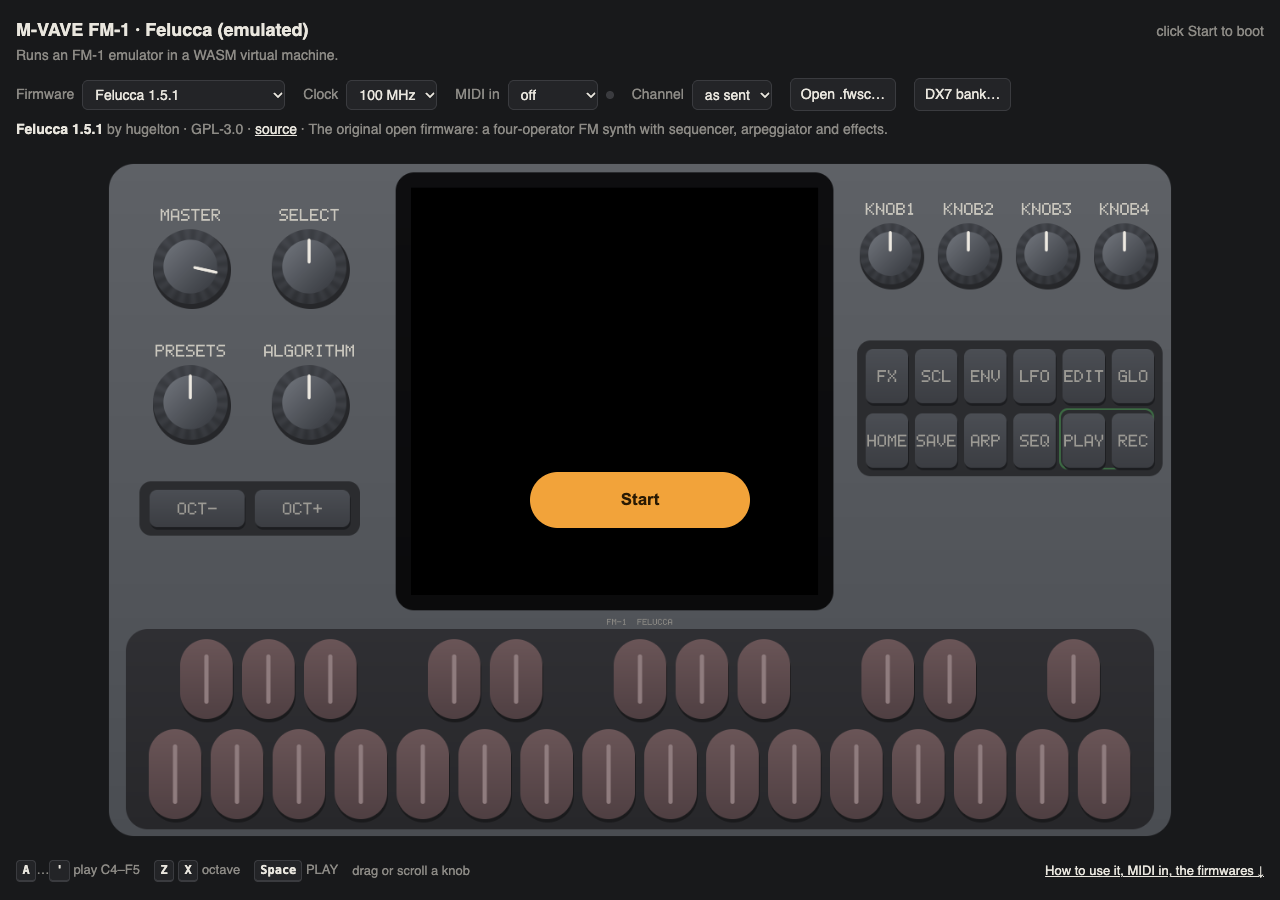
\includegraphics[width=\linewidth]{fig/page.png}
    \caption{The web page: the panel is drawn by the emulator's own code.}
  \end{subfigure}\hfill
  \begin{subfigure}[b]{0.30\textwidth}\centering
    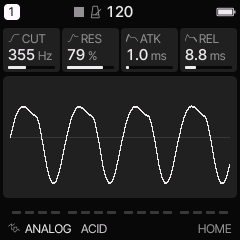
\includegraphics[width=\linewidth]{fig/felucca_lcd.png}
    \caption{The emulated LCD: Felucca~1.5.1 playing a chord, 3.0\,s after boot.}
  \end{subfigure}
  \caption{The emulator in use. The page fetches each firmware from its author's site and boots
    the same update package a real FM-1 would install.}
  \label{fig:page}
\end{figure}

\section{Starting point: reconnaissance}

The first day went to reading, not coding. The relevant public sources were: AL-255's
\emph{FM-1-RE} (boot chain, memory layout, a V13 disassembly, firmware images), ip2k's
\emph{lunar-modulator} (hardware, update protocol, recovery risks), kagaimiq's JieLi knowledge base
and tools, and Felucca's \code{hal/} directory, which is in effect the peripheral documentation:
key matrix, encoders, display, audio. Recon established that the SoC is an AC791N/WL82 (not the
``JL-BR22'' string in the firmware), that flash is 1\,MB mapped for execute-in-place at
\code{0x02000000}, and that several GPL firmwares built from C with the same toolchain exist, which
makes them golden references.

Two early checks made the plan concrete. First, AL-255's V13 disassembly was reproduced
byte-for-byte by wrapping the raw application in an ELF \code{.fw} section and running the vendor
\code{objdump} in Docker; so the vendor disassembler, not Ghidra, would be the authority on
encodings. Second, a C file compiled to pi32v2 gave (source $\rightarrow$ bytes $\rightarrow$
mnemonic) triples, e.g.\ \code{r0 += r1} = \code{10 18}, \code{rts} = \code{80 00}. The conclusion,
written into the plan on day one, was that ISA recovery would be \emph{a mining exercise, not
black-box discovery}, with differential probing as validation.

\section{Recovering the instruction set}

\begin{figure}[t]
\centering
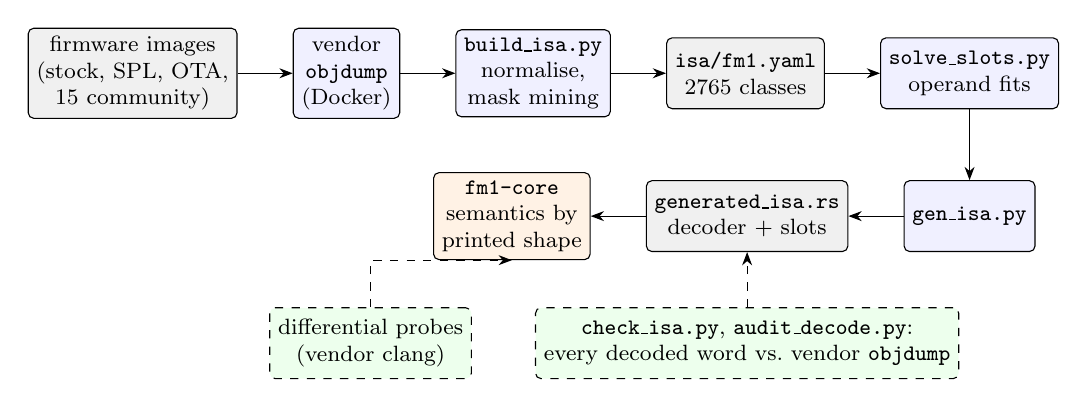
\begin{tikzpicture}[node distance=5mm and 7mm, >=Stealth,
  box/.style={draw,rounded corners=2pt,align=center,font=\footnotesize,minimum height=9mm,inner sep=3pt},
  data/.style={box,fill=black!6},
  tool/.style={box,fill=blue!6},
  chk/.style={box,fill=green!7,dashed}]
  \node[data] (fw) {firmware images\\(stock, SPL, OTA,\\15 community)};
  \node[tool,right=of fw] (od) {vendor\\\code{objdump}\\(Docker)};
  \node[tool,right=of od] (mine) {\code{build\_isa.py}\\normalise,\\mask mining};
  \node[data,right=of mine] (yaml) {\code{isa/fm1.yaml}\\2765 classes};
  \node[tool,right=of yaml] (solve) {\code{solve\_slots.py}\\operand fits};
  \node[tool,below=9mm of solve] (gen) {\code{gen\_isa.py}};
  \node[data,left=of gen] (rs) {\code{generated\_isa.rs}\\decoder + slots};
  \node[box,left=of rs,fill=orange!10] (core) {\code{fm1-core}\\semantics by\\printed shape};
  \node[chk,below=7mm of rs] (audit) {\code{check\_isa.py}, \code{audit\_decode.py}:\\every decoded word vs.\ vendor \code{objdump}};
  \node[chk,left=8mm of audit] (probe) {differential probes\\(vendor clang)};
  \draw[->] (fw)--(od); \draw[->] (od)--(mine); \draw[->] (mine)--(yaml); \draw[->] (yaml)--(solve);
  \draw[->] (solve)--(gen); \draw[->] (gen)--(rs); \draw[->] (rs)--(core);
  \draw[->,dashed] (audit)--(rs);
  \draw[->,dashed] (probe.north) |- (core.south);
\end{tikzpicture}
\caption{The ISA pipeline. The YAML table is the single source of truth: the Rust decoder is
generated from it and never edited by hand. Dashed: the checks that gate every regeneration.}
\label{fig:pipeline}
\end{figure}

\subsection{Mask mining from disassembly corpora}
The vendor \code{objdump} prints every instruction's bytes next to its text. Running it over five
corpora (the V13 and V14 applications, two bootloader builds and the USB OTA loader, about 421\,000
instructions) gives the raw material. \code{tools/build\_isa.py} normalises each line into a
\emph{printed shape}: registers become \code{R}, decimal and hex immediates \code{\#i} and
\code{\#h}, register lists are canonicalised, and the vendor's \code{<\_fw+0x...>} annotations are
stripped. (That last step had a costly bug: stripping un-anchored ate the \code{<} operator in
\code{ifs (r6 < 3) goto}, creating phantom forms that covered 3\,\% of the corpus. It is anchored at
the end of the line now.) Instructions with the same shape and length are grouped, and for each
group the bits that never vary become the class's \code{mask}/\code{match}.

The result on the first day was 1067 classes. A streaming decoder over the same corpora, choosing
by longest match, then mask popcount, then corpus count, decoded all of them with 0 mismatches and
0 undecodable words. When the fifteen community firmwares were added (their raw applications
wrapped in ELF for \code{objdump} by \code{tools/disasm\_app.sh}), the table was re-mined from 25
listings into 2765 classes; \code{tools/isa\_stable\_names.py} keeps class names stable across
re-mining because parts of the core key on them.

\subsection{Operand fields as exact linear models}
Masks say which bits are opcode; they do not say how the variable bits become operands. The first
operand fitter (\code{derive.py}) tried per-field templates and solved 206 classes. The approach
that worked, \code{tools/solve\_slots.py}, fits every printed operand of a class as an \emph{exact}
linear model over the class's varying bits, by rational Gaussian elimination, with collinear bits
resolved by a power-of-two search. Operand kinds are \code{imm}, \code{rel} (sign-extended, scaled,
pc-relative), \code{scaled}, \code{bit}/\code{nbit}, \code{composed}, \code{const}, \code{zero32} and
register blocks. A fit is accepted only if it reproduces \emph{every} sample of the class. This
raised coverage to 764 classes, 86.8\,\% of corpus instructions.

For instruction families whose encodings span several classes, \emph{family-level fitting} worked
best: take every corpus line of one printed shape across classes (e.g.\ all 5302
\code{if (rN op \#imm) goto} lines), propose the bit fields, and verify against all of them. Five
families went to zero mismatches in one session this way. Two examples of what came out:

\begin{itemize}
\item \textbf{Compare-immediate branches.} Register in bits 0--3; byte~1 selects the family
  (\code{f8} ==/!=, \code{f9} unsigned $\ge$/$<$, \code{fc} unsigned $>$/$\le$, \code{fd}/\code{fe}
  signed); bit~7 the second operator of the family; a 10-bit immediate assembled as
  bits(25,31)\,|\,bits(4,6)$\ll$7; offset $=2\cdot\mathrm{sext}_9(\ldots)$ from $pc+4$.
\item \textbf{The composed 12-bit immediate}, shared by \code{R = \#h}, \code{R = R op \#h} and
  memory read-modify-write forms. With code $c$ = bits(24,27) and $m$ = bits(16,23): $c=0$ is the
  literal $m$; 1 replicates $m$ per halfword; 2 places $m\ll8$ per halfword; 3 replicates per
  byte; $c\ge4$ is float-like, $E = 2c + (m\gg7)$, value $=(\mathtt{0x80}\,|\,(m\,\&\,\mathtt{0x7f}))\ll(32-E)$.
  This one rule reproduces a 70-entry table of observed constants (IEEE floats among them) and
  about 1650 ALU and move samples.
\end{itemize}

Bits the corpora never vary cannot be fitted from them. For those the \emph{assembler oracle} was
used: generate assembly text sweeping one operand at a time, assemble thousands of lines per Docker
run with the vendor Clang, and read the bytes back. This is how the FPU was found: the stock
firmware uses float instructions that \code{objdump} prints as \code{<unknown instruction>}; compiling
with \code{-mcpu=r3} and disassembling the assembler's output gave the \code{3f e5} encoding
(add, sub, mul, div, min, max, conversions).

\subsection{Semantics keyed by printed shape}
\code{fm1-core} executes instructions by their printed shape (\code{Cpu::exec\_syntax}), taking
operands from the generated slots in printed order, so one arm for \code{R = R + \#i} serves every
class that prints that way. Raw-bit decoders exist only where one class mixes encodings. When the
solver began covering a class, its hand-written decoder was deleted; three of those turned out to be
silently wrong (one stored \code{r9} instead of \code{r1} because it took bit~7 as part of the
register number). Behaviours established while booting real code include:

\begin{itemize}
\item \textbf{Dual-issue pairs}: an instruction printed with a trailing \code{\#} pairs with the next
  one, which reads registers from \emph{before} the first wrote them (deferred register commit).
\item \textbf{Predicated blocks} \code{if (rA op x) \{ \ldots\} else \{ \ldots\}} whose then/else
  lengths are counted in \emph{units} (a pair is one unit, a nested block one unit).
\item \textbf{Hardware loops} \code{rep N rR \{}: block length $2(\mathrm{bits}(4,7)+1)$ bytes,
  count in a register or immediate.
\item \textbf{Interrupt nesting} follows the Blackfin rule: an ISR can be interrupted only while its
  \code{reti} is saved on the stack. (Without this, a tick between an ISR's \code{reti} pop and its
  \code{rti} made the \code{rti} return to itself.)
\item \textbf{Two stacks}: in user mode an interrupt saves \code{sp} to \code{usp} and continues on
  \code{ssp}. The stock RTOS's context switch depends on it.
\item \textbf{Flags}: N, C (set means no borrow, as on ARM), Z, V in \code{psr}, read by Clang's 64-bit
  arithmetic right after the low-word add or subtract.
\end{itemize}

\section{Validation: how we knew it was right}

Without hardware, ``right'' had to be defined by things that could be checked mechanically. Four
methods were used, and every change had to pass the ones that applied.

\paragraph{1. Decoder audit against the vendor.} \code{tools/audit\_decode.py} decodes every word of a
vendor listing with the Rust decoder and compares operands with the vendor text. It found, for
instance, that a sp-relative pair store fitted on V13 alone broke for offsets $\ge 512$ (keys stayed
lit because LED arrays were stale).

\paragraph{2. Differential probes.} A probe is a small C program built with the vendor Clang in which
each check computes an expression at run time from \code{volatile} inputs and compares it with the
same expression folded at compile time by LLVM (Listing~\ref{lst:probe}). The compiler's constant
folder is thus the oracle for the compiler's own model of the ISA, and a mismatch is an emulator bug.
Probe suites cover integer arithmetic (121 checks), Felucca's Huffman font decoder on data from its
own packer (139), the FPU (1464 cases against LLVM's folding), and 64-bit and soft-double arithmetic.

\begin{lstlisting}[language=C,caption={From \code{probes/arith.c}. \code{T(runtime, folded)}: the
first argument compiles to pi32v2 instructions, the second to a constant.},label={lst:probe},captionpos=b]
volatile int32_t a = 1234567, b = -89, c = 7;
volatile uint32_t ua = 0xDEADBEEFu, uc = 13u;
T(a / c,  1234567 / 7);
T(b % c,  -89 % 7);
T(ua % uc, 0xDEADBEEFu % 13u);
T(a * 241, 1234567 * 241);
\end{lstlisting}

\paragraph{3. Same code, two machines.} Where a firmware's C source was available, a piece of it was
built both for the device and natively and compared word for word. X0X's TR-909 code exposed the
register-pair addressing modes (a pre-increment store overwrote one voice's settings with another's)
and a bitfield-extract instruction that had been executed as an add. Later, reSID's double-precision
setup computed on the emulator differed from the host; tracing it found that \code{psr} always read
0, so every 64-bit add lost its carry and every 64-bit subtract borrowed.

\paragraph{4. Byte-identical audio across execution modes.} The emulator has three ways to run the
same code: one instruction at a time (the reference), a block interpreter with micro-ops, and a JIT.
A bench mode (\code{fm1-live --bench MS} with \code{FM1\_BENCH\_WAV}, plus a scripted exercise of
every key, encoder and note) writes the raw audio. Every optimisation was accepted only if the audio
was byte-identical in all three modes \emph{and} to the build before the change, for every
firmware. This turns ``did the JIT break something subtle?'' into a file comparison. (Dual-core
firmwares are deterministic per mode but interleave cores at slightly different points, so for
them the comparison is per mode against the previous build.)

Table~\ref{tab:bugs} lists some of what these methods caught. Most bugs were invisible at the point
of failure: the symptom appeared much later, in a picture or a sound.

\begin{table}[t]
\centering\footnotesize
\begin{tabularx}{\textwidth}{@{}>{\raggedright}p{43mm}X>{\raggedright\arraybackslash}p{33mm}@{}}
\toprule
Defect & Symptom & Found by\\
\midrule
2-byte shift: bit 7 taken as register bit & CRT copy loops ran 4$\times$ too long; RAM corrupted & boot trace\\
\code{[R+\#i] = R}: bit 7 in source register & stored \code{r9} instead of \code{r1} & solver replacing hand code\\
16-bit read at word offset 2 & every 16-bit canvas sheared & probe (lcdtest)\\
unsigned compare immediates sign-extended & wrong branches on \code{if (r2 < 2111)} & probe\\
4-byte \code{R = R << \#n} run as \code{>>>} & wrong arithmetic in drawing code & probe\\
sp-relative pair offset $\ge 512$ & stale LED arrays, keys stayed lit & decoder audit\\
interrupt nesting & \code{rti} returned to itself; hang & live play\\
register-pair pre-increment modes & X0X's 909 settings overwritten & device vs.\ native build\\
\code{b4 e1} extract executed as add & an address used as an exponent & device vs.\ native build\\
no arithmetic flags & 64-bit add lost carry; reSID filter wrong & soft-double probes\\
random-number unit read as 0 & stock UI froze after 8\,s & debugging the freeze\\
unknown-access log shifted 8192 entries per access & one firmware ran far too slowly & investigating the slowdown\\
\bottomrule
\end{tabularx}
\caption{A selection of defects and how each was found.}
\label{tab:bugs}
\end{table}

\section{The system-on-chip}

\paragraph{Peripherals in boot order, lazily.} The SoC layer started with RAM, the XIP window and a
stub that logs every access to an unknown address and returns a benign value. The rule was:
\emph{the access log is the reverse-engineering roadmap}. A peripheral was modelled when a firmware
was seen to depend on it, from Felucca's HAL headers and the AC79 SDK where possible. In order:
the interrupt controller (priority nibbles, software latch, RAM vectors), TIMER4/TIMER5 on a
240\,MHz cycle clock, SPI NOR flash (fonts), an ST7789-style LCD on SPI1 with DMA, the I2S output
(ALNK0, double-buffered DMA; Felucca's samples turned out to be 24-bit words in the \emph{low}
bits, not left-justified as a HAL comment says), the SAR ADC (MASTER pot, battery), and the key
matrix behind two 74HC595 shift registers with seven quadrature encoders.

\paragraph{Felucca first, then the stock firmware.} Felucca (open source) ran end to end on day
three. The stock firmware needed more, each piece found from a concrete symptom: SPI2 DMA to scan the
key columns (keys ignored), a hardware lock between cores for \code{lockset}/\code{lockclr} (a task
queued twice), a CRC-16 unit (the patch file system failed every CRC), \code{idle} that waits for an
interrupt (0.44$\times$ real time), and a random-number generator: a routine in the audio driver
parks its task when a random word equals a fixed descrambled value, which a constant 0 always did,
so the UI froze about eight seconds after boot. The factory DX7 patch bank lives in a flash area
that updates never write; since it cannot be redistributed, a blank area gets the emulator's own
small bank, and \code{--syx} loads a DX7 bank.

\paragraph{Two cores.} The stock firmware renders sound on core 1. Core 1 starts when core 0 sets a
bit at \code{0x10008} (latched at the write: some firmwares hold it only briefly), at the address in
\code{0x01C7FFF8}. It has no clock of its own: core 0 runs in slices of 1024 instructions, then core
1 runs as many instructions as cycles passed, and stops early when it returns to the same pc with
the same registers (a job loop with nothing to do).

\section{Making it fast}

FM-1 firmwares do their audio in an interrupt every 128 samples, and live play needs the full
240\,MHz in real time. Speed was added in stages, each gated on the byte-identical audio rule:

\begin{enumerate}
\item \textbf{Decode cache} and cheap shape matching: from 1\,M to 17\,M instructions/s.
\item \textbf{Micro-ops and blocks}: common forms pre-decoded with operands and branch targets
  resolved once; straight-line blocks; RAM/XIP fast paths; idle skipping of timer-polling loops.
  Interrupt delivery stays exact at block granularity: blocks end at due ticks, peripheral writes,
  and the ends of pairs, predicated blocks and loops.
\item \textbf{AArch64 JIT} (macOS): hot blocks compiled to native code with chaining, guest state
  in the \code{Cpu} struct, inline RAM/XIP loads and stores, helpers that sync the clock to the exact
  instruction for everything else.
\item \textbf{Shrinking the slow path}: 1.7--3.8\,\% of instructions fell back to the generic path
  and cost half the time, because each also ended a block. New micro-ops (shared with the
  interpreter through one \code{exec\_raw}, so the two cannot drift), dual-issue pairs with no
  dependency run as two plain ops, and a remembered ``needs step'' marker brought it to 0.1\,\%.
\item \textbf{WebAssembly JIT}: in the browser, a hot block's \emph{region} (blocks reachable over
  fixed edges, at most 32 blocks or 384 ops) becomes a small Wasm module that the host compiles and
  installs in the exported function table; Rust calls it by index. Per-block modules gained nothing
  (blocks average 3.5 instructions); regions doubled the speed. Chrome compiles them synchronously
  inside the AudioWorklet in about 25\,\textmu s, at most 16 per audio quantum.
\end{enumerate}

\begin{table}[h]
\centering\footnotesize
\begin{tabular}{@{}lccc@{}}
\toprule
Real-time factor at 240\,MHz & slowest (X0X) & Felucca & fastest (Melodee)\\
\midrule
native, AArch64 JIT & 1.14 $\rightarrow$ 2.65 & 1.63 $\rightarrow$ 4.4 & 3.1 $\rightarrow$ 5.9\\
WebAssembly (Node) & 0.53 $\rightarrow$ 1.62 & 0.66 $\rightarrow$ 2.3 & 0.97 $\rightarrow$ 3.5\\
\bottomrule
\end{tabular}
\caption{The speed pass of day four (before $\rightarrow$ after); every firmware's bench audio
byte-identical to before.}
\label{tab:speed}
\end{table}

One measure that was tried and dropped: per-block tick accounting in the interpreter, paid before
any non-RAM access. It was 5--7\,\% slower, because blocks are short. A/B timing was done
interleaved (\code{tools/bench\_ab.sh}), since back-to-back runs drifted 6--8\,\%.

\section{The browser, MIDI and publishing}

The web build runs the emulator in an AudioWorklet. The page hosts no firmware: it fetches each
update package from its author's GitHub Pages (all allow cross-origin reads) and unpacks it with
\code{web/fwsc.js}, a package reader checked byte-equal against Felucca's own on every package.
Authors publish new versions often; when the catalog's URL is gone, the page takes the package the
author's installer page names now (four had moved on the day of publication). M-VAVE's server sends
no CORS header, so users open their own copy of the stock package.

New versions also test the emulator. On the day this report was written, Felucca~1.6 appeared and
the page picked it up; the emulator halted on \code{d7 ec 51 38}, which the vendor prints as
\code{[r5+-128] = r3}. The table had a class for it with 19 samples but no operand fit. Comparing
all word loads and stores in the 25 listings showed that bit~17 selects pre-increment or a plain
offset and that byte~0's bit~2 is the offset's sign: one model, 27\,884 samples, 0 mismatches. With
it Felucca~1.6 plays, and every other firmware's audio stayed byte-identical.

MIDI~IN is modelled at the UART, not injected into firmware: UART1 with receive DMA into a ring, a
latch that counts received bytes, and a timeout interrupt after a configured silence, one byte per
31\,250-baud byte time (320\,\textmu s). Each firmware therefore reads MIDI with its own driver;
Felucca polls the count from a timer interrupt, the stock firmware takes the timeout interrupt. The
emulator found that the stock firmware listens on channel~2, a claim still to be checked on a real
unit. In the browser, Web MIDI feeds the bytes; natively, every MIDI input of the computer.

Continuous integration runs the unit tests, builds the site and runs two smoke tests in Node
against the built WebAssembly: Felucca must boot to a screen and sound and play a MIDI note; the
SID firmware must stay silent until a key is pressed, then sound. The project began inside a
larger repository of demos and was moved into its own repository with history kept
(\code{git subtree split}); the old URLs forward with their query strings.

\section{A new firmware, developed on the emulator: FM-1 SID}

To test the emulator as a development platform, we asked whether the FM-1 could be a Commodore~64
SID synth. The study (Table~\ref{tab:sid}) compared an integer SID model written for the purpose
with reSID~0.16, reSID~1.0 and reSIDfp, by recording register streams and replaying them on every
engine, each clocked to the exact cycle of each write; the costs on the FM-1 were measured by
counting emulated instructions between markers, and the FM-1 output was compared with the host
build of the same code (bit-identical in every case).

\begin{table}[h]
\centering\footnotesize
\begin{tabular}{@{}lrrl@{}}
\toprule
Engine & instr./sample & of a 240\,MHz core & verdict\\
\midrule
own integer model & 316 & 5.8\,\% & fits; lowest fidelity\\
reSID 0.16, fast & 440 & 8.1\,\% & \textbf{fits; chosen}\\
reSID 0.16, interpolate & 5\,562 & 102\,\% & too heavy\\
reSID 0.16, resample & 39\,226 & 721\,\% & far too heavy\\
reSID 1.0 / reSIDfp & -- & -- & 8--21\,MB filter tables; FM-1 has 1\,MB flash\\
\bottomrule
\end{tabular}
\caption{SID engines per chip (3 voices and filter) at 44.1\,kHz, measured on the emulated FM-1.}
\label{tab:sid}
\end{table}

The firmware that followed nests machines: a C64 tune's own 6502 code runs in floooh's cycle-stepped
\code{m6502.h}, compiled for pi32v2, which runs on the emulated FM-1, which runs in WebAssembly in the
browser, whose hot pi32v2 code is compiled at run time into further WebAssembly. The main loop runs
the tune's play routine up to three frames ahead and queues each SID write with its C64 cycle; the
audio interrupt clocks reSID to each write's cycle. Output correlates 0.984 with host reSID fed the
same stream. The web page searches all 61\,157 tunes of the High Voltage SID Collection, fetched
from \code{hvsc.c64.org} when picked and appended to the firmware image as a ``tune pack''.

The firmware then grew into an instrument: a synth mode where the keys play twelve SID patches, a
three-track step sequencer, and an effects page (Fig.~\ref{fig:fx}) with stereo chorus, a tempo
delay whose right tap answers 1.5 times later, and a room reverb (four damped combs, two allpasses),
adapted from Felucca's effects. The same verification style applied: with effects at zero the
player's output was compared sample by sample with the firmware before the change (0 of 176\,512
samples differed); the audio interrupt's load rose from about 10\,\% to 14\,\% of the core, and RAM
use to 425 of 432\,KB. The firmware is packaged as a real FM-1 update package with Felucca's update
loader and three hash-checked files of JieLi's Apache-licensed SDK, and the package boots straight
into the synth mode. The firmware image, rebuilt on macOS through the Dockerised toolchain, was
byte-identical to the one built on Linux.

Writing this firmware found four more emulator defects (the flags and carry gaps of
Table~\ref{tab:bugs} among them), which is itself an argument for developing against an emulator
whose every fix comes with a probe.

\begin{figure}[t]
\centering
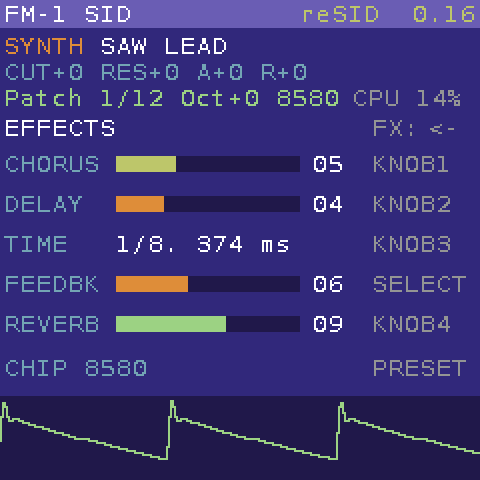
\includegraphics[width=0.36\textwidth]{fig/fxpage.png}
\caption{FM-1 SID's effects page on the emulated LCD: the knob assignments, the delay time computed
from the sequencer tempo, the chip model, and an oscilloscope of the output.}
\label{fig:fx}
\end{figure}

\section{How the work was organised}

\begin{table}[t]
\centering\footnotesize
\begin{tabularx}{\textwidth}{@{}lX@{}}
\toprule
Day & Result\\
\midrule
1 (Oct 8) & Recon; toolchain verified in Docker; V13 disassembly reproduced byte-for-byte.\\
2 (Oct 9) & 1067 classes mined, operand solver (86.8\,\% of instructions); stock V13 boots to RTOS start on two cores.\\
3 (Oct 10) & Interrupts, timers, flash, LCD, I2S, keys: Felucca plays; live at 240\,MHz with the AArch64 JIT; fifteen firmwares, the FPU, the browser build, published.\\
4 (Oct 11) & Flags and carry; stock firmware with both cores; SID study, player firmware, HVSC page, synth mode, update package, sequencer; WebAssembly JIT.\\
5 (Oct 12) & MIDI in; a guide on the page; own repository; FM-1 SID boots as a synth, with effects.\\
\bottomrule
\end{tabularx}
\caption{Timeline. The repository has 38 commits; each is a working state that passed the checks.}
\label{tab:time}
\end{table}

The work was done by one person directing an AI coding agent (Claude Code, Anthropic). The division
of labour was roughly as follows. The human chose what to build and in which order (the emulator
itself, the SID synth idea, adding effects, booting the SID firmware as a synth, moving to a
repository of its own), judged results by playing and listening, decided the tone of the public
pages (``a better story'', less technical), and approved anything outward-facing: pushes, publishing,
messages to others. The agent read the sources, ran the vendor toolchain, wrote the mining and
fitting tools, the emulator, the probes and the firmware, measured, and kept a running work log
(\code{PLAN.md}) that recorded each phase's state, numbers and open questions, so that work could
resume after an interruption or in a new session. Separate agents were occasionally used for
self-contained jobs, such as writing the page's guide.

What made the agent's output trustworthy was not review of every line but a small set of rules that
turned claims into checks:

\begin{itemize}
\item \textbf{One source of truth.} The decoder is generated from the YAML table; a second,
  hand-maintained table was never allowed. When generated slots covered a class, the hand-written
  decoder was deleted, which is how three silent bugs surfaced.
\item \textbf{The oracle is the vendor, not a guess.} Encodings are checked against the vendor
  disassembler; semantics against the vendor compiler's constant folding; unseen bits against the
  vendor assembler.
\item \textbf{Byte-identical or it did not happen.} Optimisations must leave audio unchanged across
  execution modes and against the previous build, for every firmware.
\item \textbf{Log the unknown, never swallow it.} Unknown memory accesses are logged, unknown
  instructions halt with their class name; both are to-do lists.
\item \textbf{State what is unverified.} Statements not yet checked on hardware (the stock MIDI
  channel, FM-1 SID on a real unit, which instructions set flags) are marked as such in the
  documentation and on the pages.
\end{itemize}

\section{Limitations}

Nothing here has yet been compared with a real FM-1. Instruction timing is one cycle per instruction
except where peripherals impose waits; flash wait states and divide latency are not modelled.
Which instructions update flags on the real core is assumed from compiled code, which only reads
them right after a producer. Two FPU operations in the stock firmware (codes 7 and 8) are unknown.
The real entry chain of core 1 is not understood; the emulator starts it at the address the
firmware writes. These are the first things to test once the hardware arrives: running the
differential probes on the device would turn the emulator's assumptions into measurements.

\section{Conclusion}

An undocumented CPU in a consumer device turned out to be recoverable from its firmware in days,
because the vendor's own tools could serve as oracles: the disassembler for encodings, the assembler
for bits the corpora never vary, and the compiler's constant folding for semantics. The rest was
engineering discipline: a generated decoder, peripherals modelled on demand from an access log, and a
byte-identical audio rule that let aggressive optimisation (two JITs) proceed without fear. The
result runs every published FM-1 firmware in a browser, and was good enough to develop a new
firmware on before the synth was on the desk.

\section*{Acknowledgements}
Built on the community's work: AL-255's FM-1-RE, ip2k's lunar-modulator, kagaimiq's jielie,
hugelton's Felucca (whose hardware layer and effects FM-1 SID uses), cicloid's awesome-fm-1, and every
firmware author who published their work. reSID is by Dag Lem; \code{m6502.h} by Andre Weissflog;
the SID tunes come from the High Voltage SID Collection.

\begin{thebibliography}{9}\small
\bibitem{fm1re} AL-255. \emph{FM-1-RE}. \url{https://github.com/AL-255/FM-1-RE}
\bibitem{lunar} ip2k. \emph{lunar-modulator}. \url{https://github.com/ip2k/lunar-modulator}
\bibitem{jielie} kagaimiq. \emph{jielie}. \url{https://kagaimiq.github.io/jielie}
\bibitem{felucca} hugelton. \emph{Felucca}. \url{https://github.com/hugelton/Felucca}
\bibitem{awesome} cicloid. \emph{awesome-fm-1}. \url{https://github.com/cicloid/awesome-fm-1}
\bibitem{resid} D.~Lem. \emph{reSID}, version 0.16.
\bibitem{chips} A.~Weissflog. \emph{chips} (\code{m6502.h}). \url{https://github.com/floooh/chips}
\bibitem{hvsc} \emph{High Voltage SID Collection}. \url{https://hvsc.c64.org}
\bibitem{emu} J.~Eriksson. \emph{fm1-emu}. \url{https://github.com/joakimeriksson/fm1-emu}
\end{thebibliography}

\end{document}
